% latexmk -pvc -pdf
\documentclass[9pt, a4paper]{article}
\usepackage[margin=0.65in]{geometry}
\usepackage{graphicx}
\usepackage{caption}
\usepackage{amsmath,amsthm,amsfonts,amssymb}
\usepackage{blindtext}
\usepackage[english]{babel}
\newenvironment{Figure}
    {\par\medskip\noindent\minipage{\linewidth}}
    {\endminipage\par\medskip}

\title{Simulating phase contrast imaging for materials with variable density (PART II)}
\author{Ana C. Fabela Hinojosa \\
\small{Supervisors: Assoc. Prof. Marcus Kitchen}}
\small{\date{\today,  \\Due date: Friday 23\textsuperscript{th} September, 2021}}

\begin{document}
\maketitle
\section{Current objective}
In this project I study the theoretical perspective of coherent X-ray imaging by creating several simulations of cylinder shaped sample materials subject to different energy X-ray wave-fields. In some of my simulations I use a single cylinder made of a monomorphic material and in others I use two embedded concentric cylinder shaped samples of materials with either an equal chemical composition and different densities or different chemical composition and the same density. 
My simulation's goal is to verify if and how distinctly phase contrast occurs from a sample of two different brain material samples of grey and white matter under the same wave-field. and whether the observed phase contrast is density dependent. The aim is to verify if successful phase retrieval can be done of the imaged objects given variable sample material densities.

\section{Theory fundamentals}

For my single monomorphic material cylinder simulations I use the projection approximation to solve a partial differential equation known as the transport-of-intensity equation (TIE). This equation is used to quantify the contrast (i.e. refractive (phase) effects) present in propagation-based X-ray phase contrast images\cite{PagsTutes}.
\begin{equation}\label{eq:1}
-\nabla_{T} [I(x, y, z) \nabla_{T} \phi(x, y, z)] = k \frac{\partial I (x, y, z)}{\partial z}.
\end{equation}
where $k$ is the wave-number, $I(x, y, z)$ is the intensity and $\phi(x, y, z)$ is the phase of the X-ray beam.
The projection approximation takes into account X-ray--matter interaction, therefore the position dependent and complex form for the refractive index is introduced: $n(x, y, z) = 1 - \delta(x, y, z) + i \beta(x, y, z)$. The real part of this complex quantity corresponds to the refractive index while the imaginary part is related only to the absorptive properties  properties of the imaged sample\cite{PagsTutes}.
In the projection approximation, the Beer-Lambert law of attenuation is used to relate the intensity attenuation to the physical properties of the sample
\begin{equation}\label{eq:2}
I(x, y, z_0) = \mathrm{exp}[-\int_{t} \mu(x, y, z) dz] I(x, y, 0),
\end{equation}
where $\mu = 2k\beta$ is the \textit{linear attenuation coefficient} of the sample, a function of the imaginary part of the sample's complex refractive index.
The projection approximation term involving the refractive index decrement $\delta$ physically describes phase-shifts of each wave-front coordinate which continuously accumulate in the direction of the light propagation.
\begin{equation}\label{eq:3}
\Delta \phi(x, y) = -k \int_{t}\delta(x, y, z)dz,
\end{equation}
where $t$ is the projected thickness of the object in the direction of the light flow.
The TIE effects observable changes onto the intensity equation (\ref{eq:2}) and phase equation (\ref{eq:3}) after these are used as the initial conditions of the propagation problem.

% <<<MORE RK DEETS?>>>

For my two cylinder simulations I also use the projection approximation but this time I model the propagation of the X-ray monochromatic wave-field using a method known as the angular spectrum formulation (ASF) to produce phase contrast images. This method uses Fourier decomposition of wave-fields at a single plane into distinct component plane waves. Each plane wave component is propagated through the Fourier domain to a destination plane and then the propagated wave-field components are reconstructed via an inverse spatial Fourier transform\cite{Goodman}. To implement the ASF I used the X-ray imaging group XRI library, since their algorithm has already implemented several fixes to undesirable instabilities that can appear in the simulations. 

\subsection{Imaging brain materials}
Current knowledge about the properties of grey and white matter is that they are optically extremely similar. However, it is known that there is a small difference in the values of the attenuation coefficients of these materials. In previous work done by my supervisor and other members of the X-ray imaging group, CT brain imaging has been reported to yield clearly demarcated tissue borders at the grey/white matter boundaries\cite{Beltran2}. I want to verify whether X-ray imaging grey and white matter can also yield visible phase contrast fringes. My goal is to verify if the observed boundaries in Beltran et al.(2011) (see reference \cite{Beltran2}) are due to a density difference between grey and white matter, or whether the boundaries are solely due to the materials being chemically different.

To simulate grey and white matter I used the attenuation coefficients${\mu_{GM,WM}}$ obtained by CT imaging data acquired at Japan's SPring-8 synchrotron radiation facility using an X-ray energy of $E = 24$keV and a sample-to-detector distance of $5$m\cite{Linda}. I also obtained some experimental grey and white matter densities reported in the ``IT’IS Database for thermal and electromagnetic parameters of biological tissues".To find the complex refractive index components of the whole brain (i.e. $\delta_B$ and $\mu_B$) under certain energy X-rays, I used the X-ray imaging group ``X-ray attenuation calculator" which uses the NIST values in recorded in database 66\cite{NIST} (note: I used this specific tool in all my simulations, not only the ones pertaining the brain materials). 
Using all these tools I calculated an approximate estimate for the grey and white matter corresponding refractive index decrements ($\delta_{GM}$ and $\delta_{WM}$) as either proportional to the ratio of the attenuation coefficient value for the full brain from reference\cite{NIST} and the density of the grey or white matter values reported in reference \cite{ITIS} (i.e. $\delta_{GM,WM} = \frac{\mu_B}{\rho_{GM,WM}} \delta_B$) or solely proportional to the ratio between the attenuation coefficient value for the full brain and the corresponding grey or white matter attenuation coefficient value (i.e. $\delta_{GM,WM} = \frac{\mu_B}{\mu_{GM,WM}} \delta_B$). 

\section{Current results}
\subsection{Simulating a single monomorphic cylinder}
I solved the TIE in two-dimensions using the projection approximation to establish my initial conditions. My method used a fourth order Runge-Kutta evolution algorithm to propagate the intensity and phase of the monochromatic scalar electromagnetic wave-field over a distance of 1 meter. Originally my code discretised a two-dimensional space as an x array with 1024 points and a y array with 512 points. I first attempted to solve the TIE in Fourier space. To calculate the wave-field's derivative terms in equation (\ref{eq:1}) I used the Fourier derivative theorem to write the derivatives. I also defined functions describing the geometry and optical properties (i.e. refractive index: $\delta(x, y, z)$ and $\mu(x, y, z)$) of the simulated cylinder. Both $\delta$ and $\mu$ functions used a sigmoid function with adjustable gradient to slightly blur the edge of the cylinder and avoid instability while solving the integrals in equations (\ref{eq:2}) and (\ref{eq:3}). My method was slow due to the Fourier derivatives and the output intensity profile after propagation did not appear very stable. I adjusted the ratio of the spacings in my discretised space several times to make sure that the Nyquist mode of the TIE was resolved adequately. Eventually I managed to get a smooth looking intensity profile.
\begin{Figure}
\centering
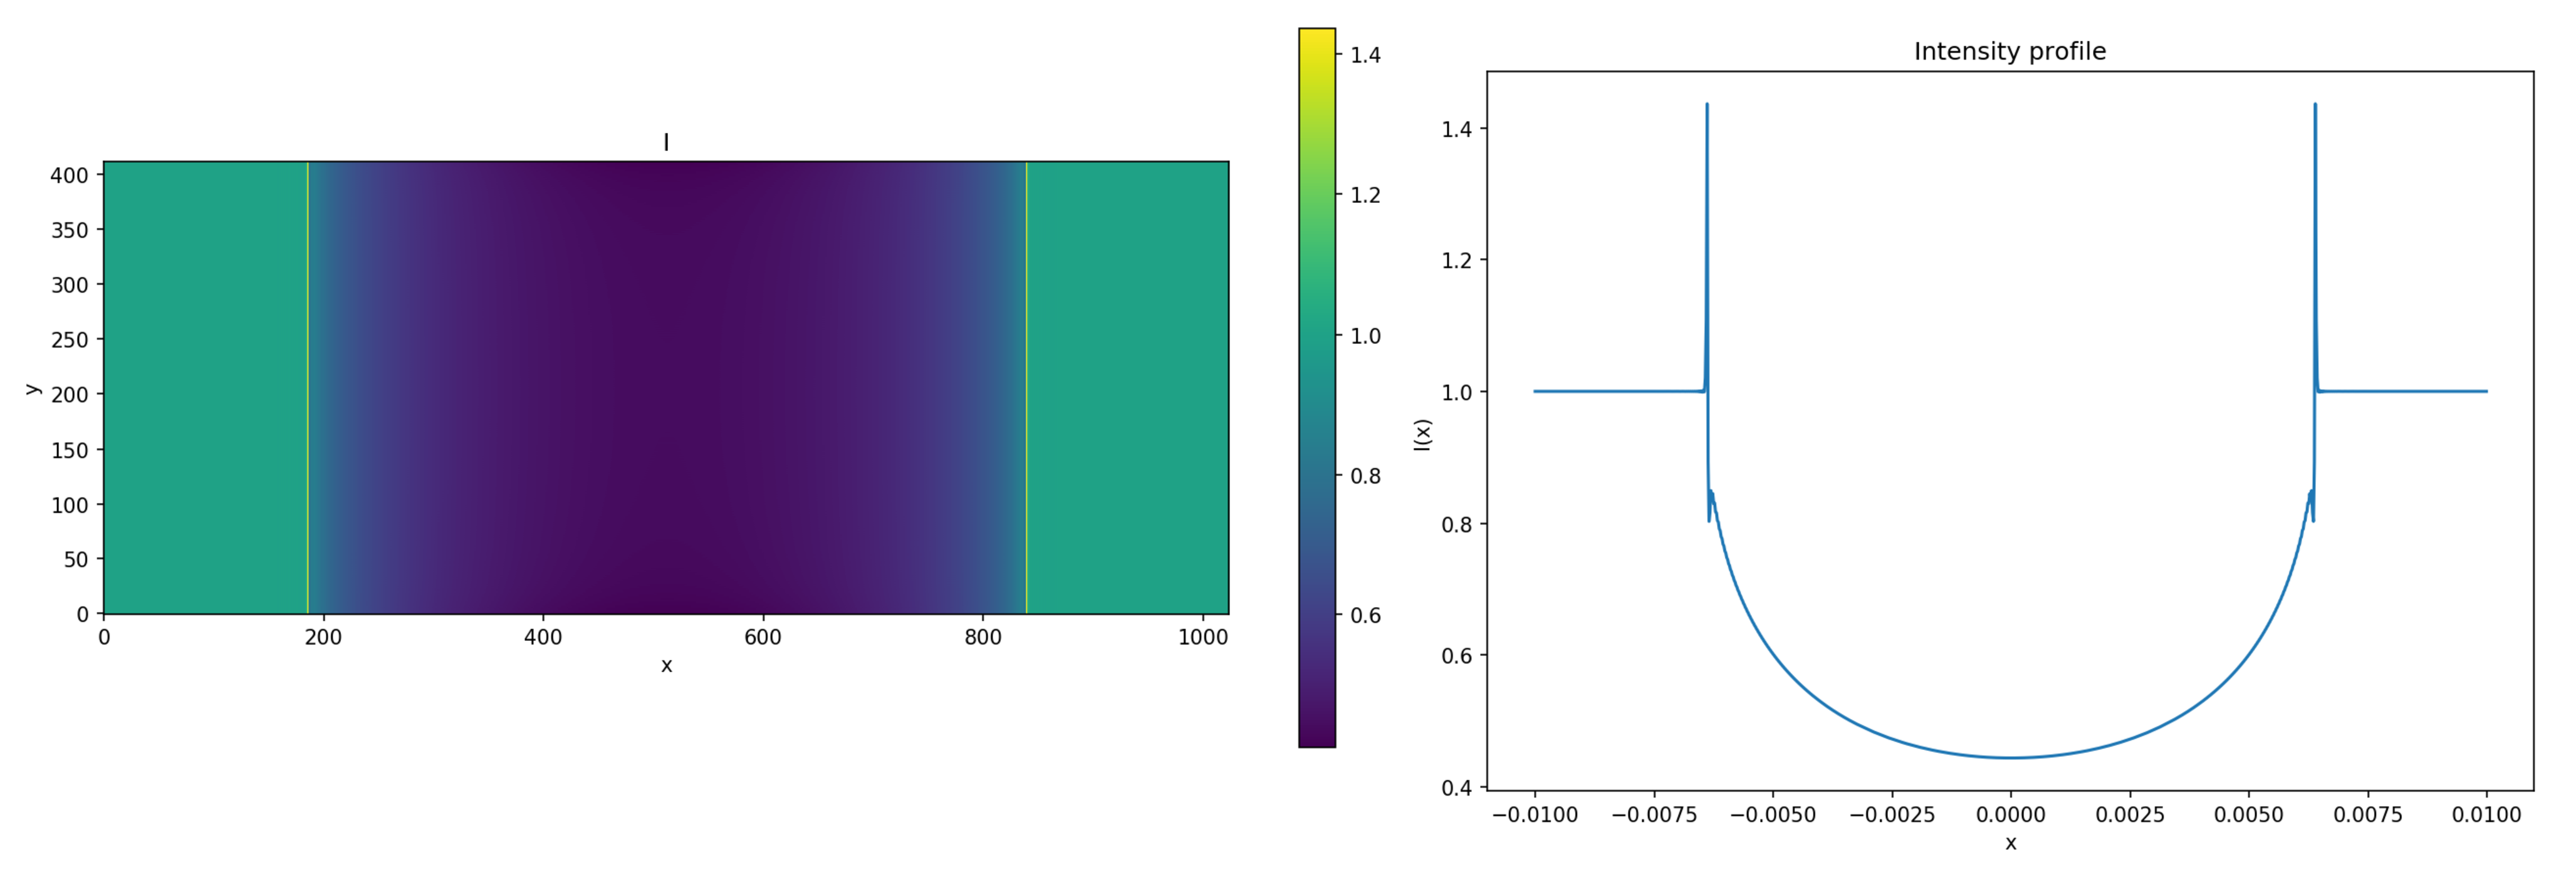
\includegraphics[width=\linewidth]{Fourier_intensity_profile.pdf}
\captionof{figure}{This phase contrast image and phase contrast cross section were the best results I obtained from my Fourier TIE method. Unfortunately my Fourier method was not able to simultaneously match the expected phase contrast peak height given this energy and sample material parameters while at the same time remaining stable. The parameters used to obtain this image were an X-ray energy equal to $22.1629$keV (corresponding to a Ag k-alpha 1 source), the cylinder's material was water which has a refractive index decrement $\delta = 468.141$nm while the attenuation coefficient is $\mu = 64.38436\mathrm{m^{-1}}$. The cylinder's radius was $R = 6.375$mm. The sigmoid function blurred $0.5$ pixels over the edge of the imaged cylinder. The propagation distance used was $z = 1$m.}
\end{Figure}

After obtaining this result I decided partially to change my approach and at the suggestion of my supervisor I solved the TIE in position space with finite differences. I used \texttt{numpy.gradient} for the derivative terms and \texttt{scipy.ndimage.laplace} for the phase Laplacian term in the TIE. This time my code discretised the two-dimensional space as an x and a y array each with 1024 points. 
After these changes I was able to understand the probable underlying reason why my Fourier method didn't work even though in theory it should have, given that it is accurate to infinite order\cite{Chris}\cite{Fornberg}. The issue was due to an effect known as Gibbs phenomenon, this effect occurs when the nth partial sum of a Fourier series undergoes large oscillations near regions with jump discontinuities\cite{Gibbs}. Discovering that higher degree polynomial interpolation does not always improve accuracy was interesting and certainly unexpected.
\begin{Figure}
\centering
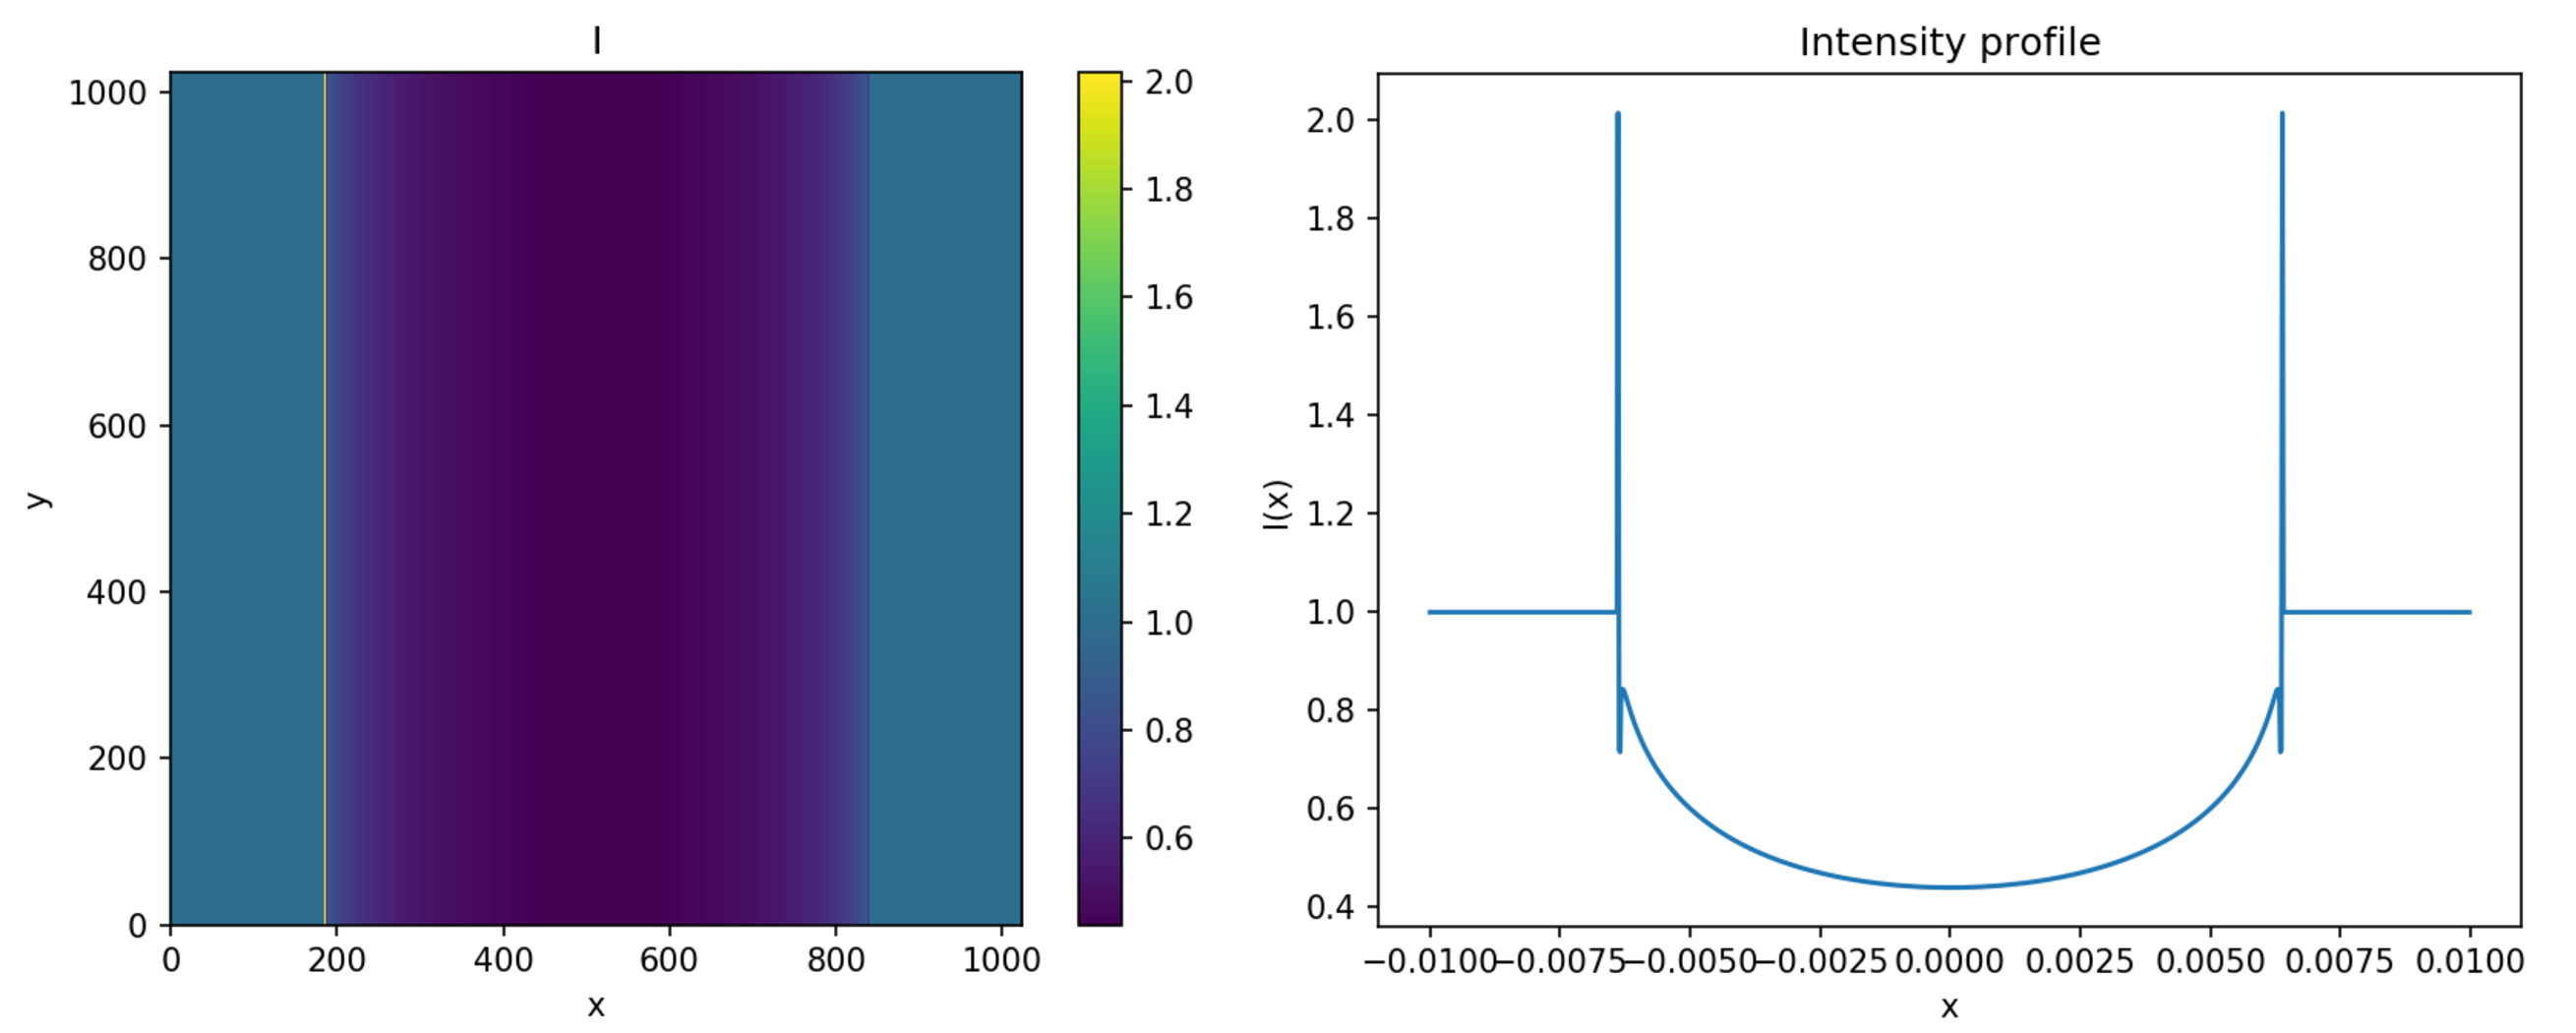
\includegraphics[width=\linewidth]{FD_intensity_profile.pdf}
\captionof{figure}{This phase contrast image and phase contrast cross section were obtained using my Finite differences and Runge-Kutta propagation method . As it can be seen here the phase contrast peaks are much higher than the profile found using the Fourier method. The parameters used to obtain this image were an X-ray energy equal to $22.1629$keV (corresponding to a Ag k-alpha 1 source), the cylinder's material was water which has a refractive index decrement $\delta = 468.141$nm while the attenuation coefficient is $\mu = 64.38436\mathrm{m^{-1}}$. The cylinder's radius was $R = 6.375$mm. The sigmoid function blurred $0.14$ pixels over the edge of the imaged cylinder. The propagation distance used was $z = 1$m. The apparent asymmetry of the two-dimensional phase contrast image is due to aliasing.}
\end{Figure}
This result actually presented an apparent improvement in the height of the expected phase contrast fringes. I decided to test my code more thoroughly and made sure that all input parameters were the same as those used in the code my supervisor provided me with to do some output comparisons.

\subsection{Testing if Runge-Kutta propagation increases phase contrast}
\begin{Figure}
\centering
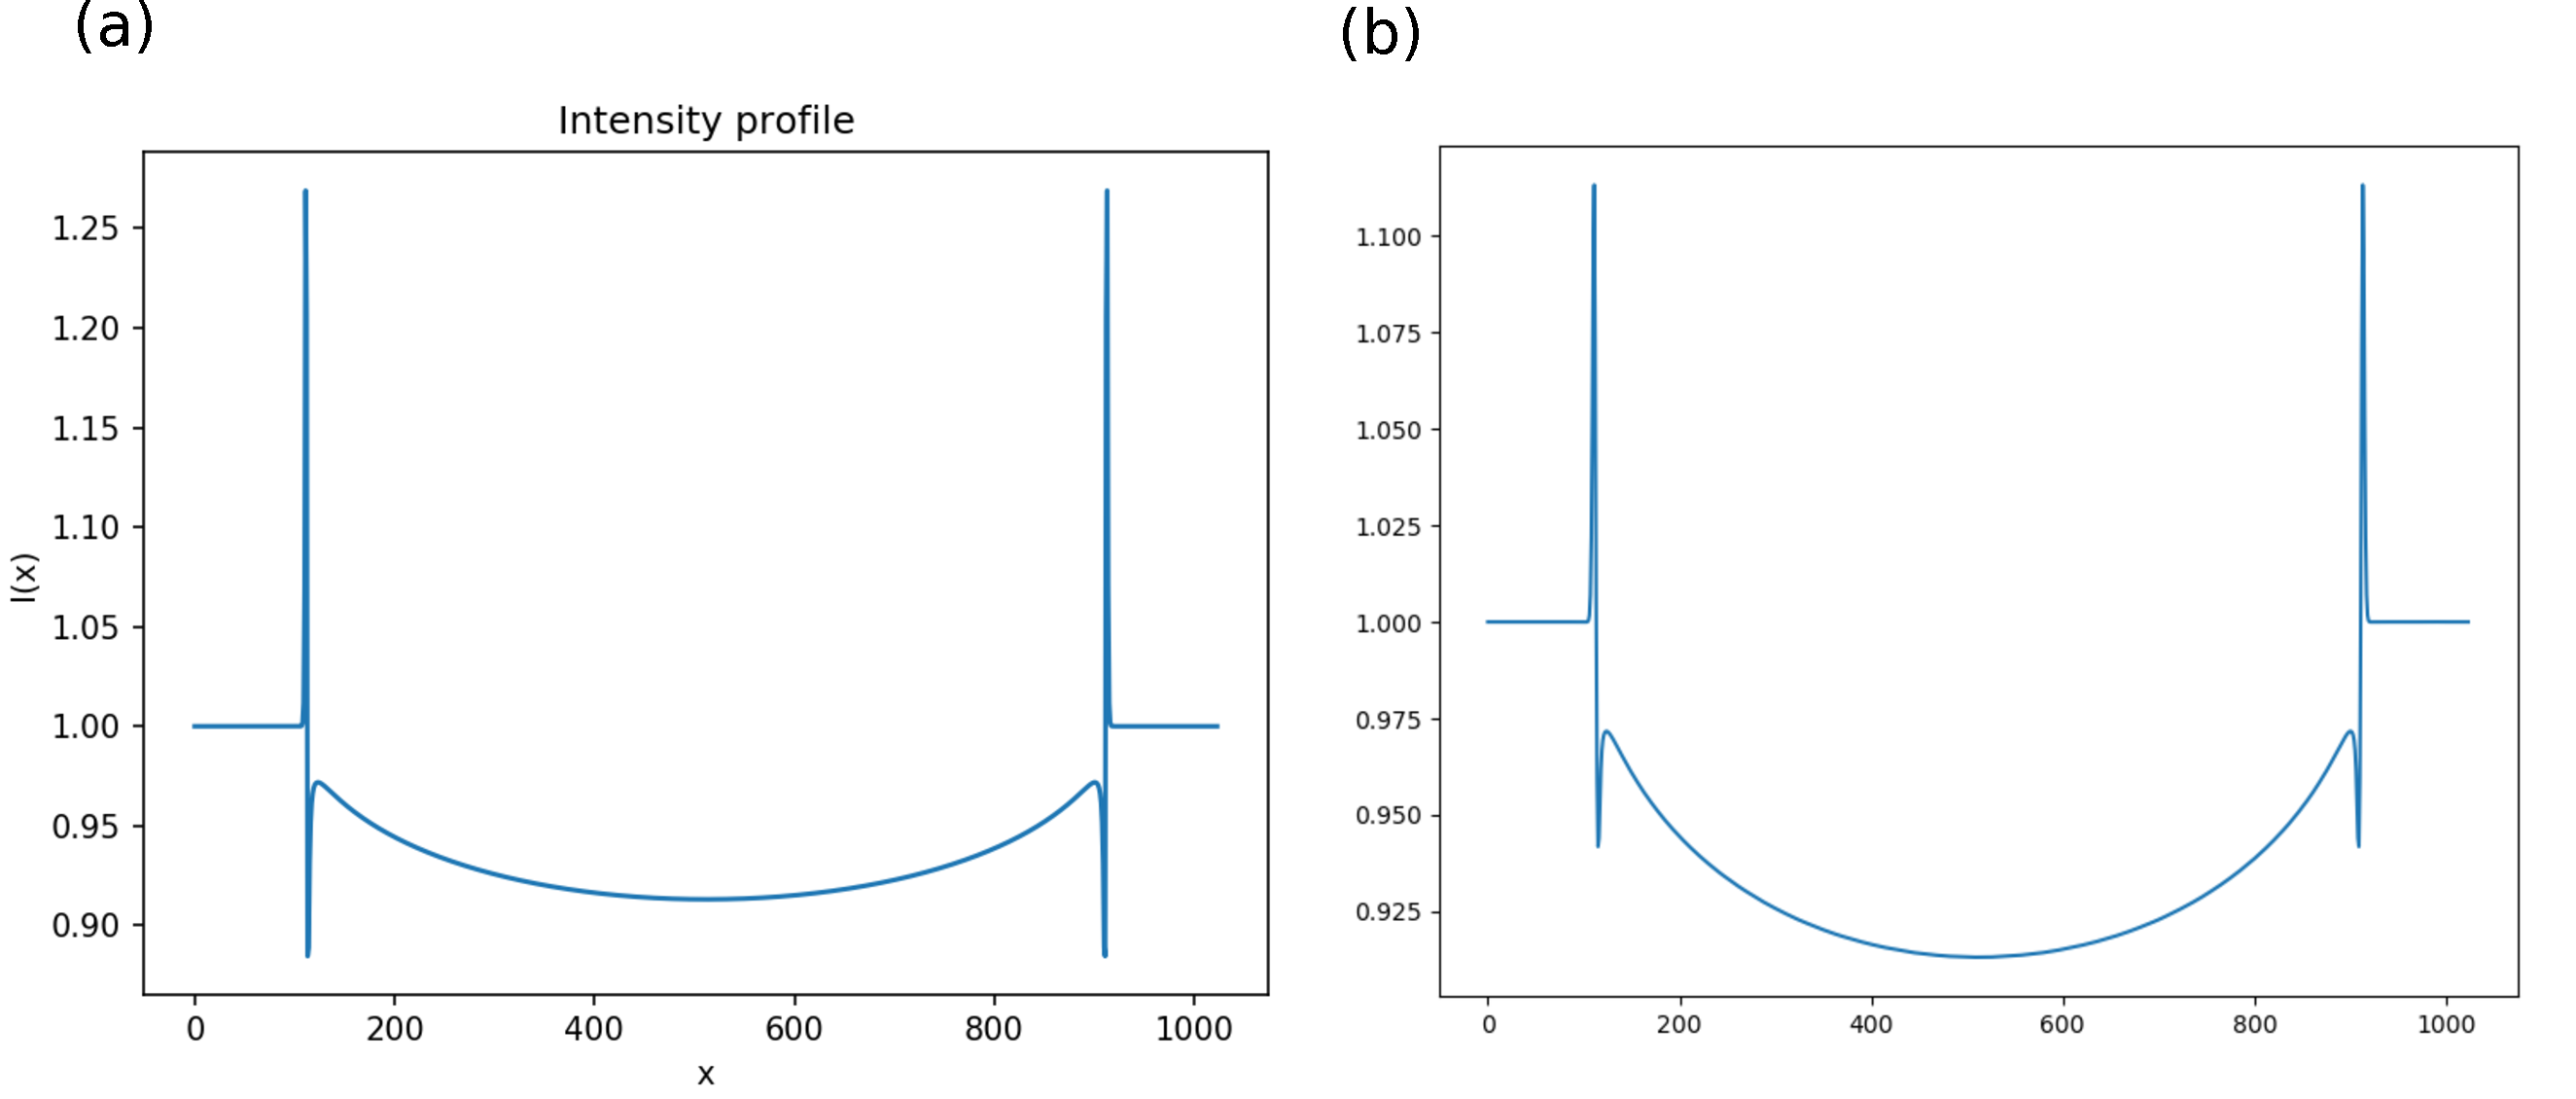
\includegraphics[width=\linewidth]{RK_TEST.pdf}
\captionof{figure}{These phase contrast cross sections were obtained by testing: (a) my Finite differences and Runge-Kutta propagation method and (b) the angular spectrum formulation method as the \texttt{xri.sim.propAS()} function created by the X-ray imaging group. The input parameters and spatial discretisation codes were identical in both (a) and (b) tests. The parameters were for a single cylinder with a radius of  $R = 2$mm. The sample material was water at a density of $1\mathrm{gcm^{-3}}$ and the X-ray energy used was $50$keV. I used the ``X-ray attenuation calculator" to find the refractive index decrement $\delta = 92.1425$nm and an attenuation coefficient $\mu = 22.69615\mathrm{m^{-1}}$. In Figure (a), the sigmoid function blurred $0.14$ pixels over the edge of the imaged cylinder.  
The spatial discretisation arrays used in (a) and (b) were x and y arrays of size $1024$ each and of pixel size $5\mathrm{\mu}$m. The propagation distance used was $z = 1$m.}
\end{Figure}

\subsection{Simulating a couple of concentric monomorphic cylinders}

\subsubsection{Density difference test: Water and Ice}
To test the density dependence of phase contrast I first used a couple embedded concentric sample of two cylinders with the outer most one made of water and the inner most one made of ice.
\begin{Figure}
\centering
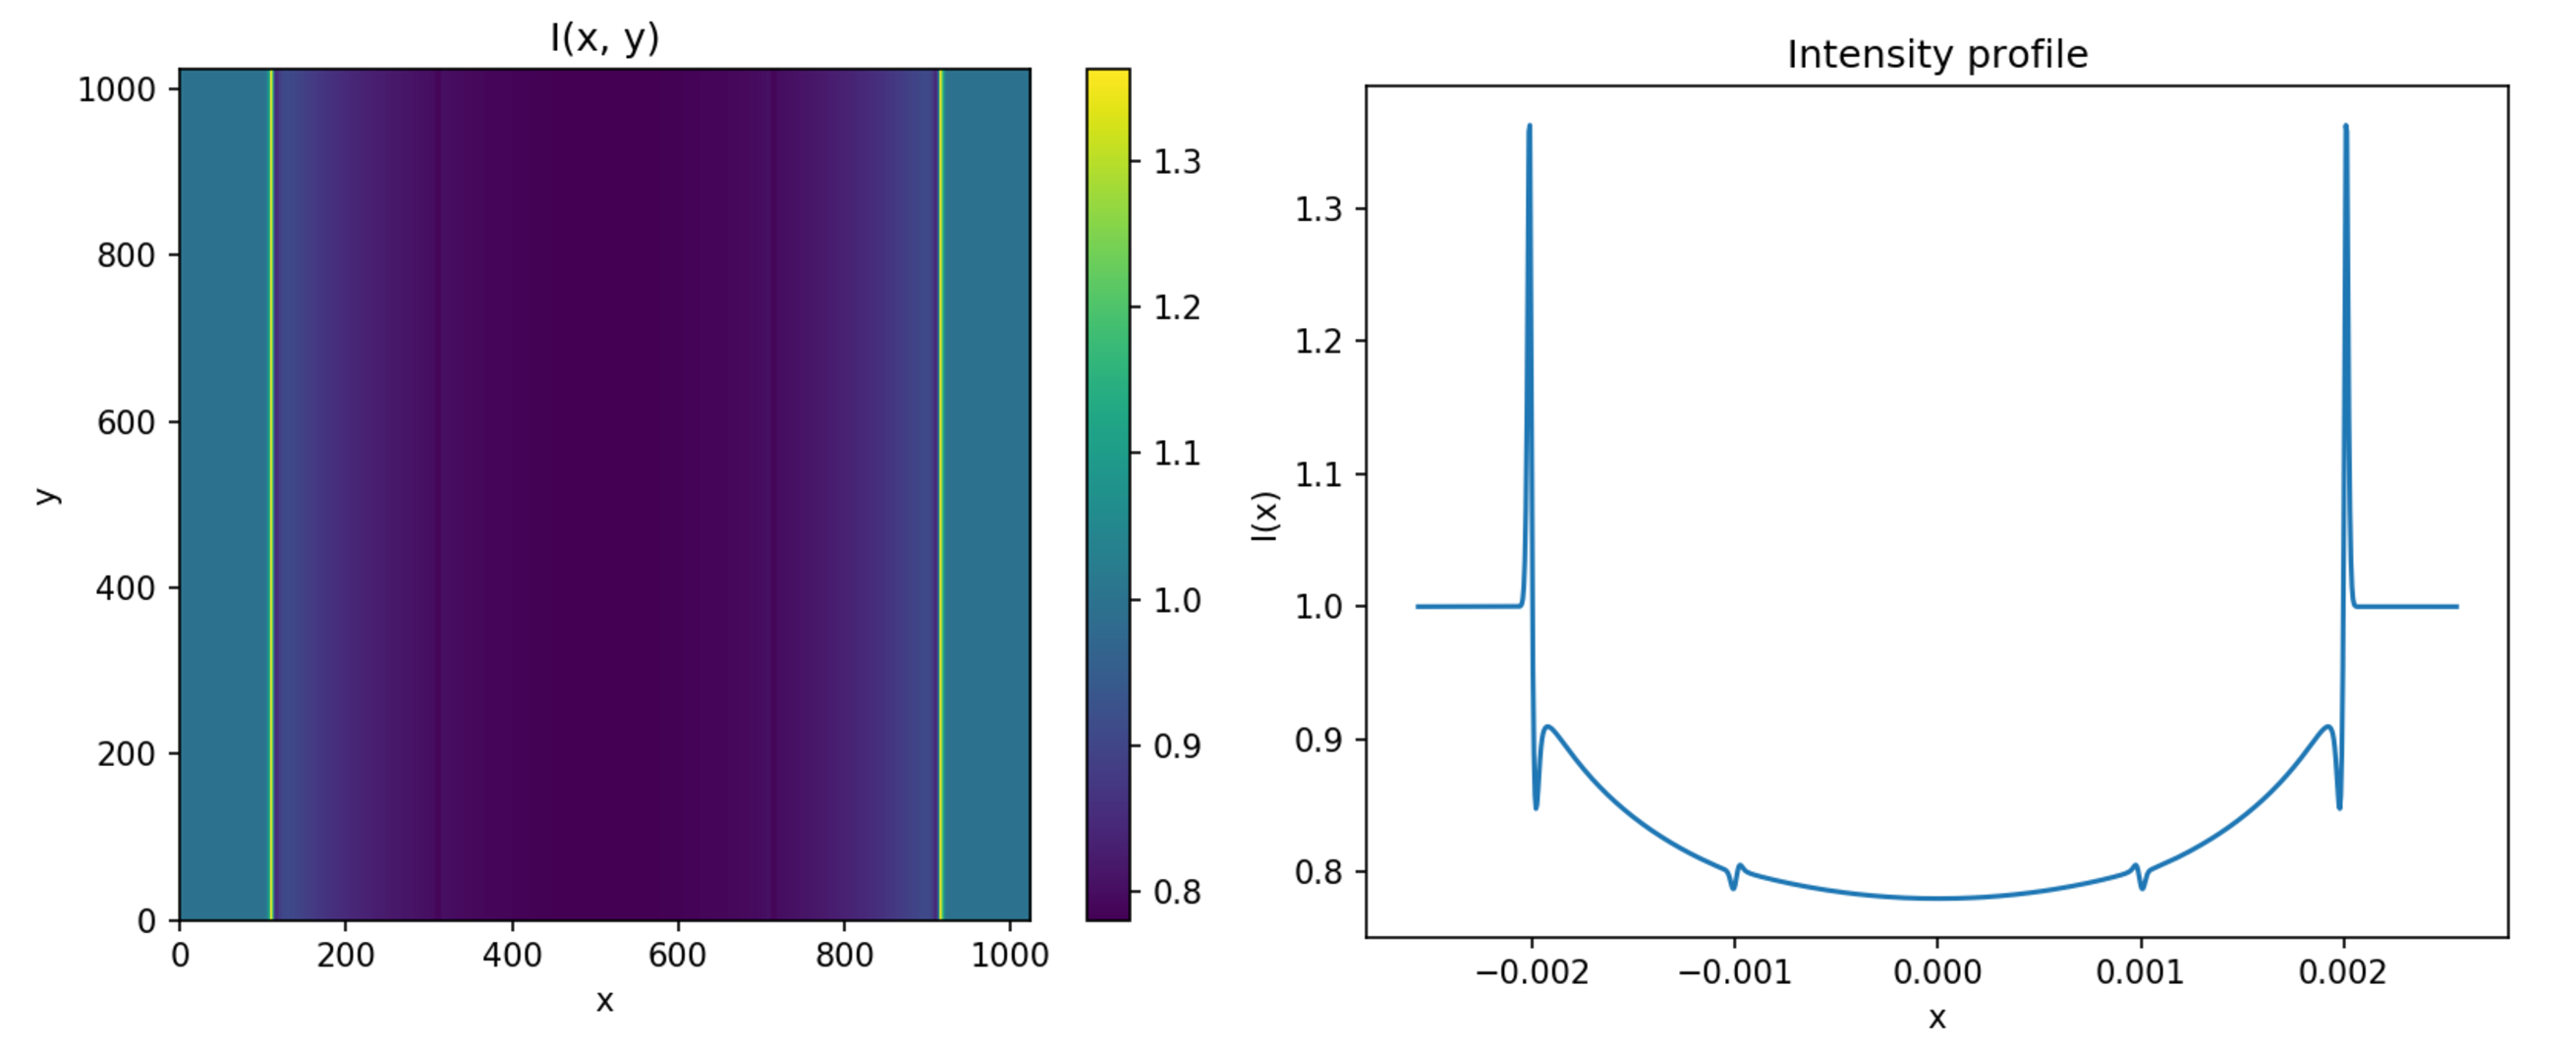
\includegraphics[width=\linewidth]{ice_water_AS.pdf}
\captionof{figure}{This phase contrast image and phase contrast cross section were obtained with the angular spectrum formulation method as the \texttt{xri.sim.propAS()} function created by the X-ray imaging group. The X-ray energy used in this simulation was $E = 22.1629$keV. The water cylinder has a refractive index decrement $\delta_W = 469.337$nm, under this energy the attenuation coefficient of water is $\mu_W = 64.55083\mathrm{m^{-1}}$. The ice cylinder has a refractive index decrement $\delta_I = 431.790$nm and attenuation coefficient $\mu_I = 59.38677\mathrm{m^{-1}}$. The density difference between these materials is $\Delta \rho = 0.08\mathrm{g cm^{-3}}$. The cylinder's radii were $R_W = 2$mm and $R_W = 1$mm. The propagation distance used was $z = 2.5$m.}
\end{Figure}

Another simulation I made for this test takes into account the apparatus parameters and the resolution of the detector used in my supervisors lab. The plan is to test these results experimentally.
\begin{Figure}
\centering
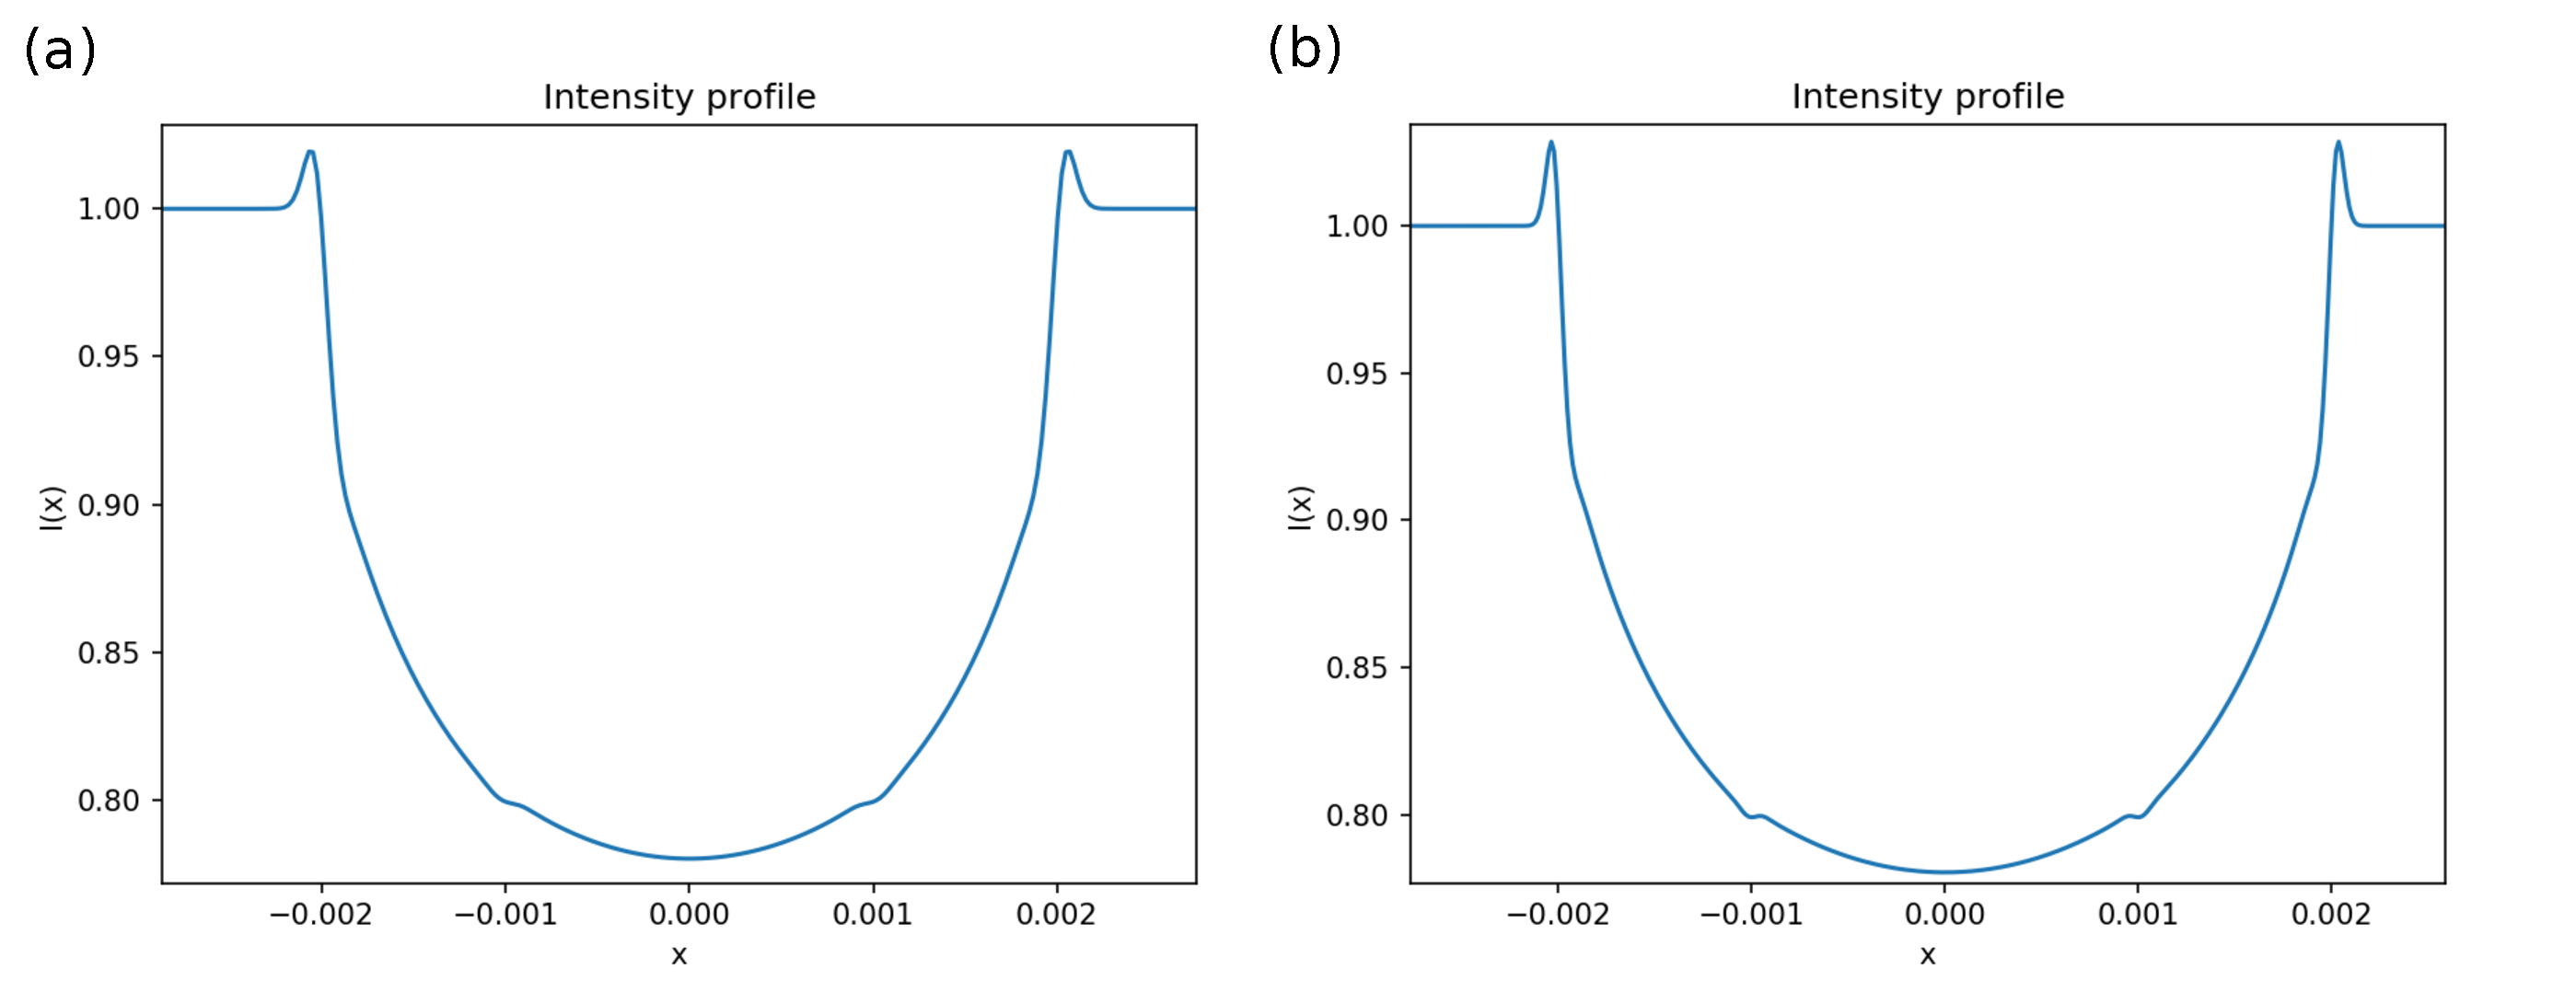
\includegraphics[width=\linewidth]{LAB_ice_water_AS_2_magnifications.pdf}
\captionof{figure}{This phase contrast cross section was obtained with most parameters being equal to those in the simulation above, except that this time I made some conversions in the spatial discretisation parameters (i.e. x and y arrays), for the conversions I took account the most likely magnification factors we would use for figure 4(a) the magnification factor is $2.5$X, for figure 4(b)the magnification factor is $4.0$X. I made sure that the dimensions of the spatial arrays and the pixels I used in this simulations matched those of the photon counting detector we will use in the lab. doing this guarantees that the pixels in the object plane are adequately sized given the expected size of the pixels in the detector plane. The effective propagation distance is also inversely scaled by the magnification.}
\end{Figure}

\subsubsection{Density difference test: Grey matter and white matter}
In this simulation I assume that grey and white matter have the same chemical compositions but distinct densities
\begin{Figure}
\centering
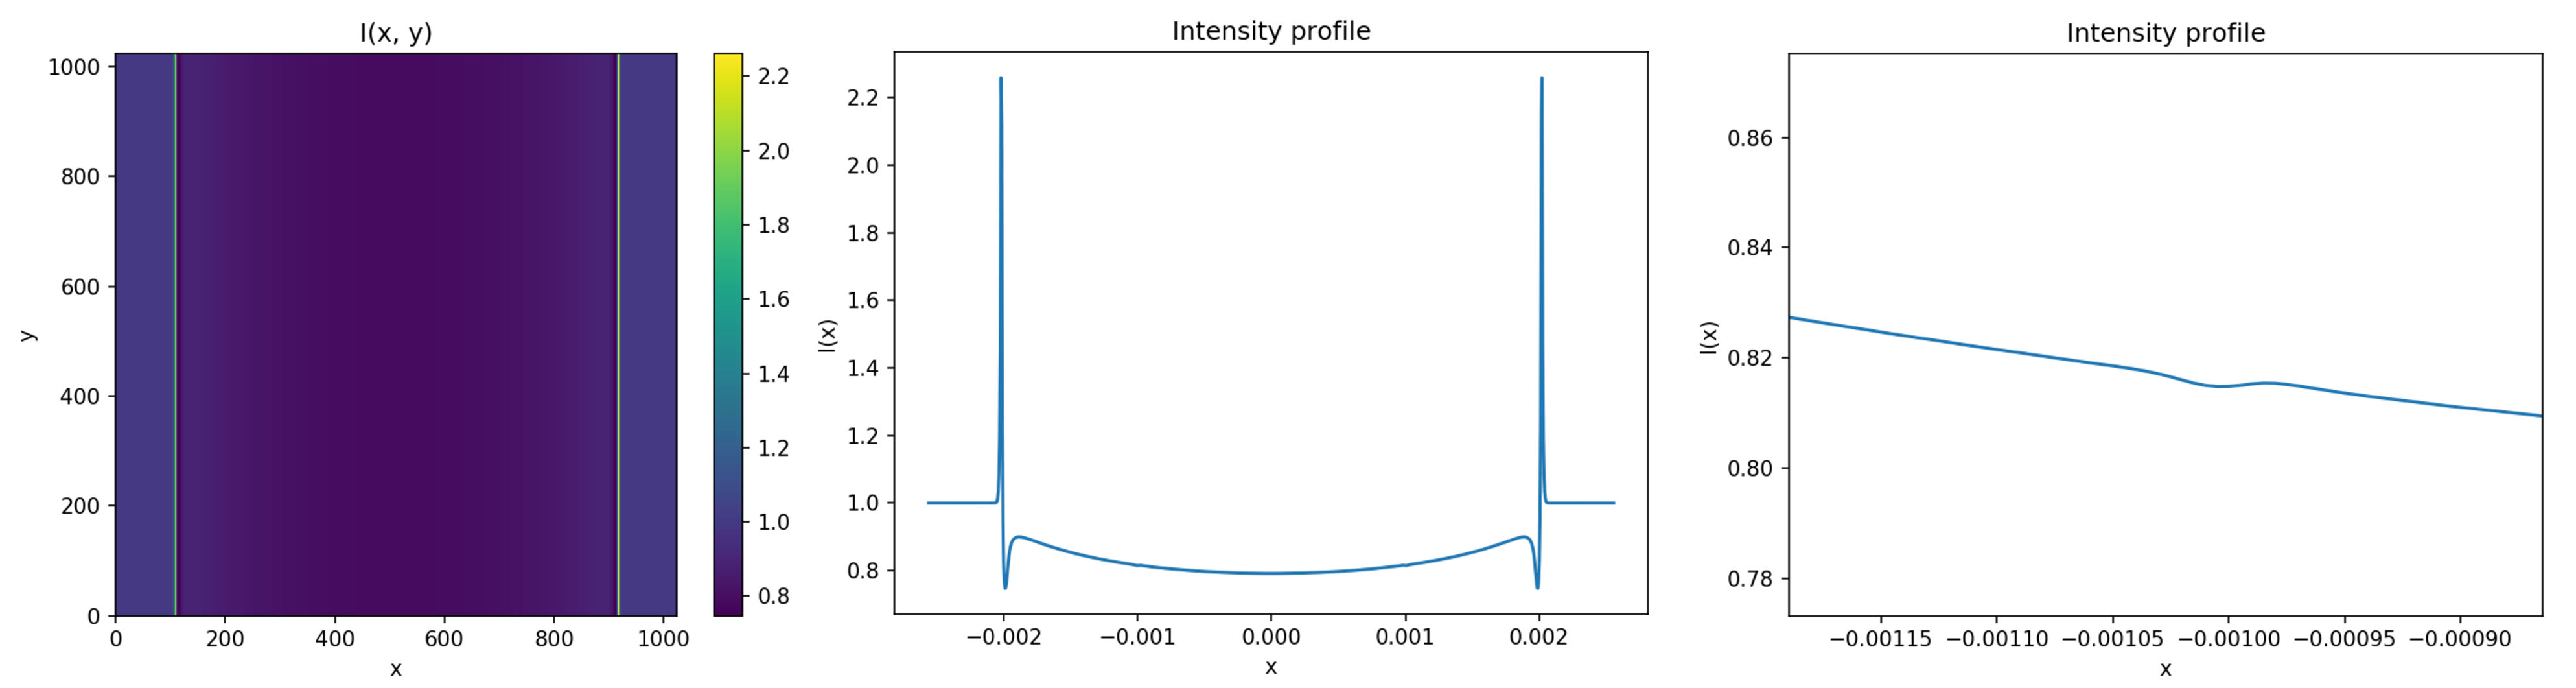
\includegraphics[width=\linewidth]{pessimistic_case.pdf}
\captionof{figure}{This phase contrast image and phase contrast cross section were obtained with the angular spectrum formulation method as the \texttt{xri.sim.propAS()} function created by the X-ray imaging group. The X-ray energy used in this simulation was $E = 24$keV. The water cylinder has a refractive index decrement $\delta_{GM} = 413.45$nm, under this energy the attenuation coefficient of grey matter is $\mu_{GM} = 58.2978\mathrm{m^{-1}}$. The white matter cylinder has a refractive index decrement $\delta_{WM} = 411.87$nm and attenuation coefficient $\mu_{GM}= 58.0747\mathrm{m^{-1}}$. The density difference between these materials is $\Delta \rho = 0.08\mathrm{g cm^{-3}}$. The cylinders' radii were $R_{GM} = 2$mm and $R_{WM} = 1$mm. The propagation distance used was $z = 2.5$m.}
\end{Figure}

\subsubsection{Chemical difference test: Grey matter and white matter}
\begin{Figure}
\centering
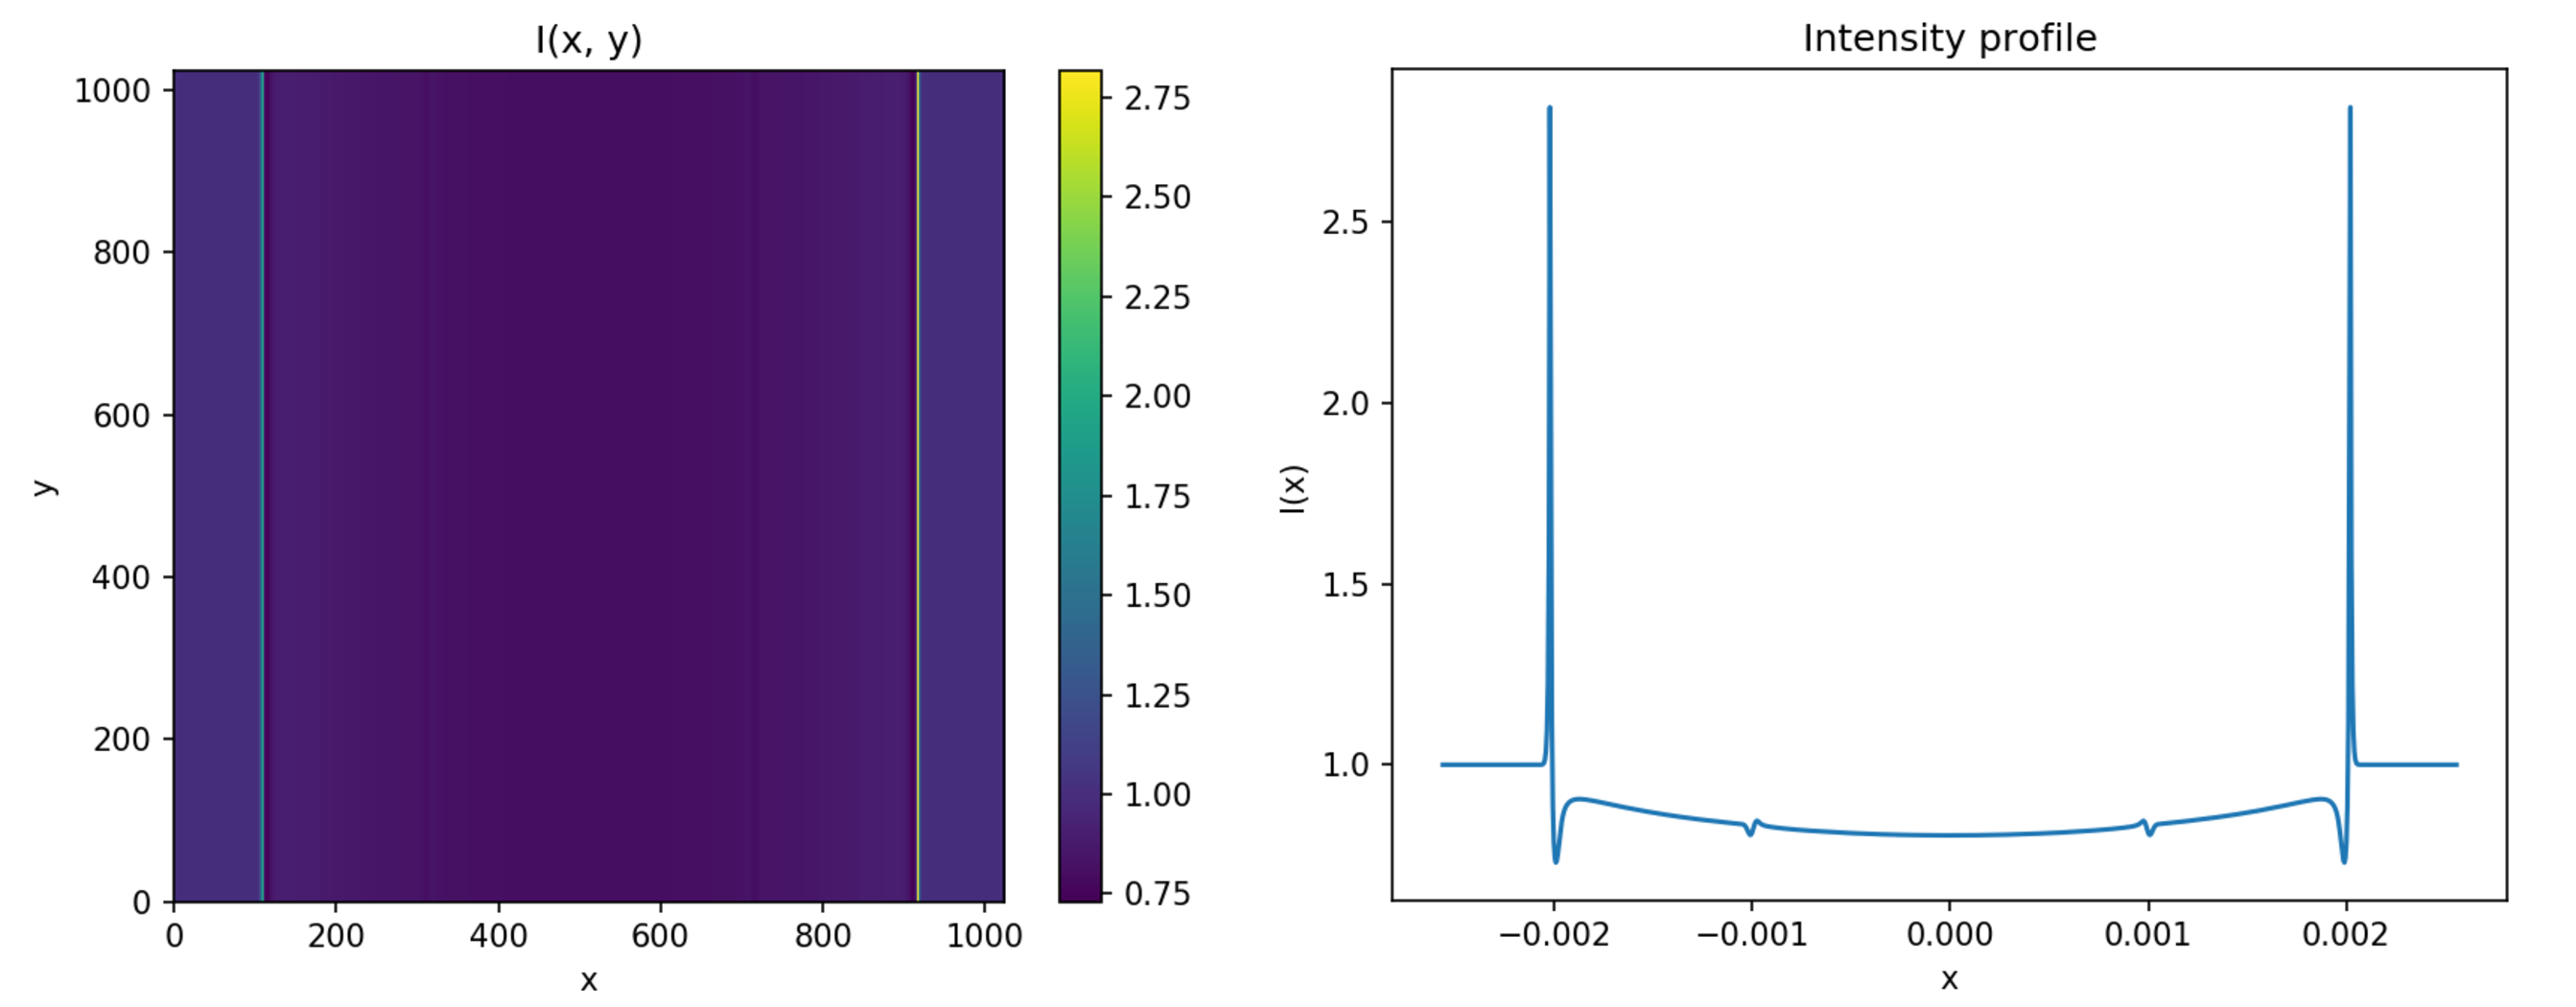
\includegraphics[width=\linewidth]{optimistic_case.pdf}
\captionof{figure}{This phase contrast image and phase contrast cross section were obtained with the angular spectrum formulation method as the \texttt{xri.sim.propAS()} function created by the X-ray imaging group. The pase contrast fringes from the inner cylinder are extremely small but can still be observed. The X-ray energy used in this simulation was $E = 24$keV. The water cylinder has a refractive index decrement $\delta_{GM} = 459.1$nm, under this energy the attenuation coefficient of grey matter is $\mu_{GM} = 52\mathrm{m^{-1}}$. The white matter cylinder has a refractive index decrement $\delta_{WM} = 426.31$nm and attenuation coefficient $\mu_{GM}= 56\mathrm{m^{-1}}$. The cylinders' radii were $R_{GM} = 2$mm and $R_{WM} = 1$mm. The propagation distance used was $z = 2.5$m.}
\end{Figure}

To do these two tests I verified that the my calculated theoretical and experimental $\mu$ values of grey and white matter do not match. Which lead me to find distinct values of $\delta$ for both tests. This mismatch was probably because in the density difference case test the assumption is that there are no chemical differences at all between grey and white matter but this is likely not true. 
My supervisor and I decided that I should continue using the chemical difference test parameters in future simulations, because this data will help compensate for chemical composition differences. I will have to test the density difference case further with these parameters.

\section{Future Plans}

My supervisor and I are planning to verify my simulation results for the water and ice case in his lab as soon as possible.

I aim to finish my simulation by creating a graphic user interface (GUI) that allows the user to modify interactively the density parameters of the imaged concentric cylinders in the simulation. The goal is to make a easily operated visual representation of the changes in phase and intensity of the X-rays as they interact with the object in-situ.

In the foreseeable future my supervisor and I plan to diversify my project by making me do some simulations about a topic known as speckle analysis. A speckle pattern is commonly produced by interference of coherent light wave-fronts as these transmit through or reflect from a random phase assigning object (scattering medium), the process is known to encode information about the scattering medium that created the speckle\cite{Specks}. The main goal of making me do the speckle simulations is for me to understand the possible sources and causes of speckles in X-ray imaging, and to be able to decode speckle patterns.

% I also plan to aid my supervisor with testing a newly obtained silver target source of X-rays for his lab apparatus. I aim to do data analysis to compare the results from the new silver target to the classic tungsten target used in the apparatus currently.

\section{Conclusion}
The present aim of my project is to test in a lab some phase contrast simulations I created to investigate how the phase of incident X-rays changes as the density of a couple of distinct sample materials in an arbitrary imaging system changes. The eventual goal of this simulation is to verify if successful phase retrieval can be done of the imaged objects given their variable densities. In this report I present a brief outline of the theoretical perspective of coherent X-ray imaging, a description of my current progress and future aims.

\bibliography{mybib}
\bibliographystyle{unsrt}
\end{document}
